\documentclass[tikz,border=10pt]{standalone}
\usepackage{pgfplots}
\pgfplotsset{compat=1.17}

\begin{document}
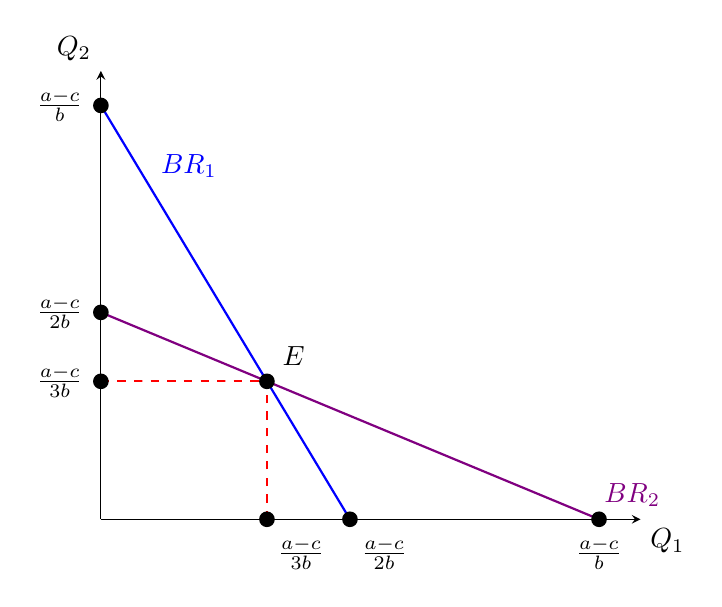
\begin{tikzpicture}
\begin{axis}[
    axis lines=left,
    xlabel={$Q_1$},
    ylabel={$Q_2$},
    ymin=0, ymax=13,
    xmin=0, xmax=13,
    xtick=\empty, 
    ytick=\empty,
    clip=false,
    xlabel style={at={(ticklabel* cs:1)},anchor=north west},
    ylabel style={at={(ticklabel* cs:1)},anchor=south east, rotate=-90},
    every axis plot/.append style={thick},
]

% Reaction Curve Firm 1
\addplot[domain=0:6, color=blue] {12-2*x} node[pos=.2, anchor=south west] {$BR_1$};
\addplot[domain=0:12, color=violet] {6-0.5*x} node[pos=.99, anchor=south west] {$BR_2$};

% Dashed lines to E
\addplot[domain=0:4, color=red, dashed] {4};% node[pos=1.1] {};
\addplot[color=red, dashed] coordinates {(4,0) (4,4)};

% % Dashed lines to M
% \addplot[domain=0:3, color=teal, dashed] {3};% node[pos=1.1] {};
% \addplot[color=teal, dashed] coordinates {(3,0) (3,3)};

% % Dashed lines to PC
% \addplot[domain=0:6, color=orange, dashed] {6};% node[pos=1.1] {};
% \addplot[color=orange, dashed] coordinates {(6,0) (6,6)};


% Labels
% y-axis
\node[label={180:{\( \frac{a-c}{b} \)}},circle,fill,inner sep=2pt] at (axis cs:0,12) {};
\node[label={180:{\( \frac{a-c}{2b}\)}},circle,fill,inner sep=2pt] at (axis cs:0,6) {};
\node[label={180:{\( \frac{a-c}{3b}\)}},circle,fill,inner sep=2pt] at (axis cs:0,4) {};
% \node[label={180:{\( \frac{a-c}{4b}\)}},circle,fill,inner sep=2pt] at (axis cs:0,3) {};
% x-axis
\node[label={270:{\( \frac{a-c}{b} \)}},circle,fill,inner sep=2pt] at (axis cs:12,0) {};
\node[label={280:{\( \frac{a-c}{2b}\)}},circle,fill,inner sep=2pt] at (axis cs:6,0) {};
\node[label={280:{\( \frac{a-c}{3b}\)}},circle,fill,inner sep=2pt] at (axis cs:4,0) {};
% \node[label={270:{\( \frac{a-c}{4b}\)}},circle,fill,inner sep=2pt] at (axis cs:3,0) {};
% on the graph
\node[label={45:{\( E \)}},circle,fill,inner sep=2pt] at (axis cs:4,4) {};
% \node[label={225:{\( M \)}},circle,fill,inner sep=2pt] at (axis cs:3,3) {};
% \node[label={45:{\( PC \)}},circle,fill,inner sep=2pt] at (axis cs:6,6) {};

\end{axis}
\end{tikzpicture}
\end{document}
